% !TeX program = xelatex
% !TeX encoding = UTF-8
% !TeX root    = document_template.tex
\documentclass{../mirea-prog-lang}

\usepackage{hyperref}
\hypersetup{pdftitle={Шаблон для mirea-prog-lang}, pdfauthor={В. С. Верхотуров}}

\usepackage{graphicx}
\usepackage{pdfpages}

\begin{document}

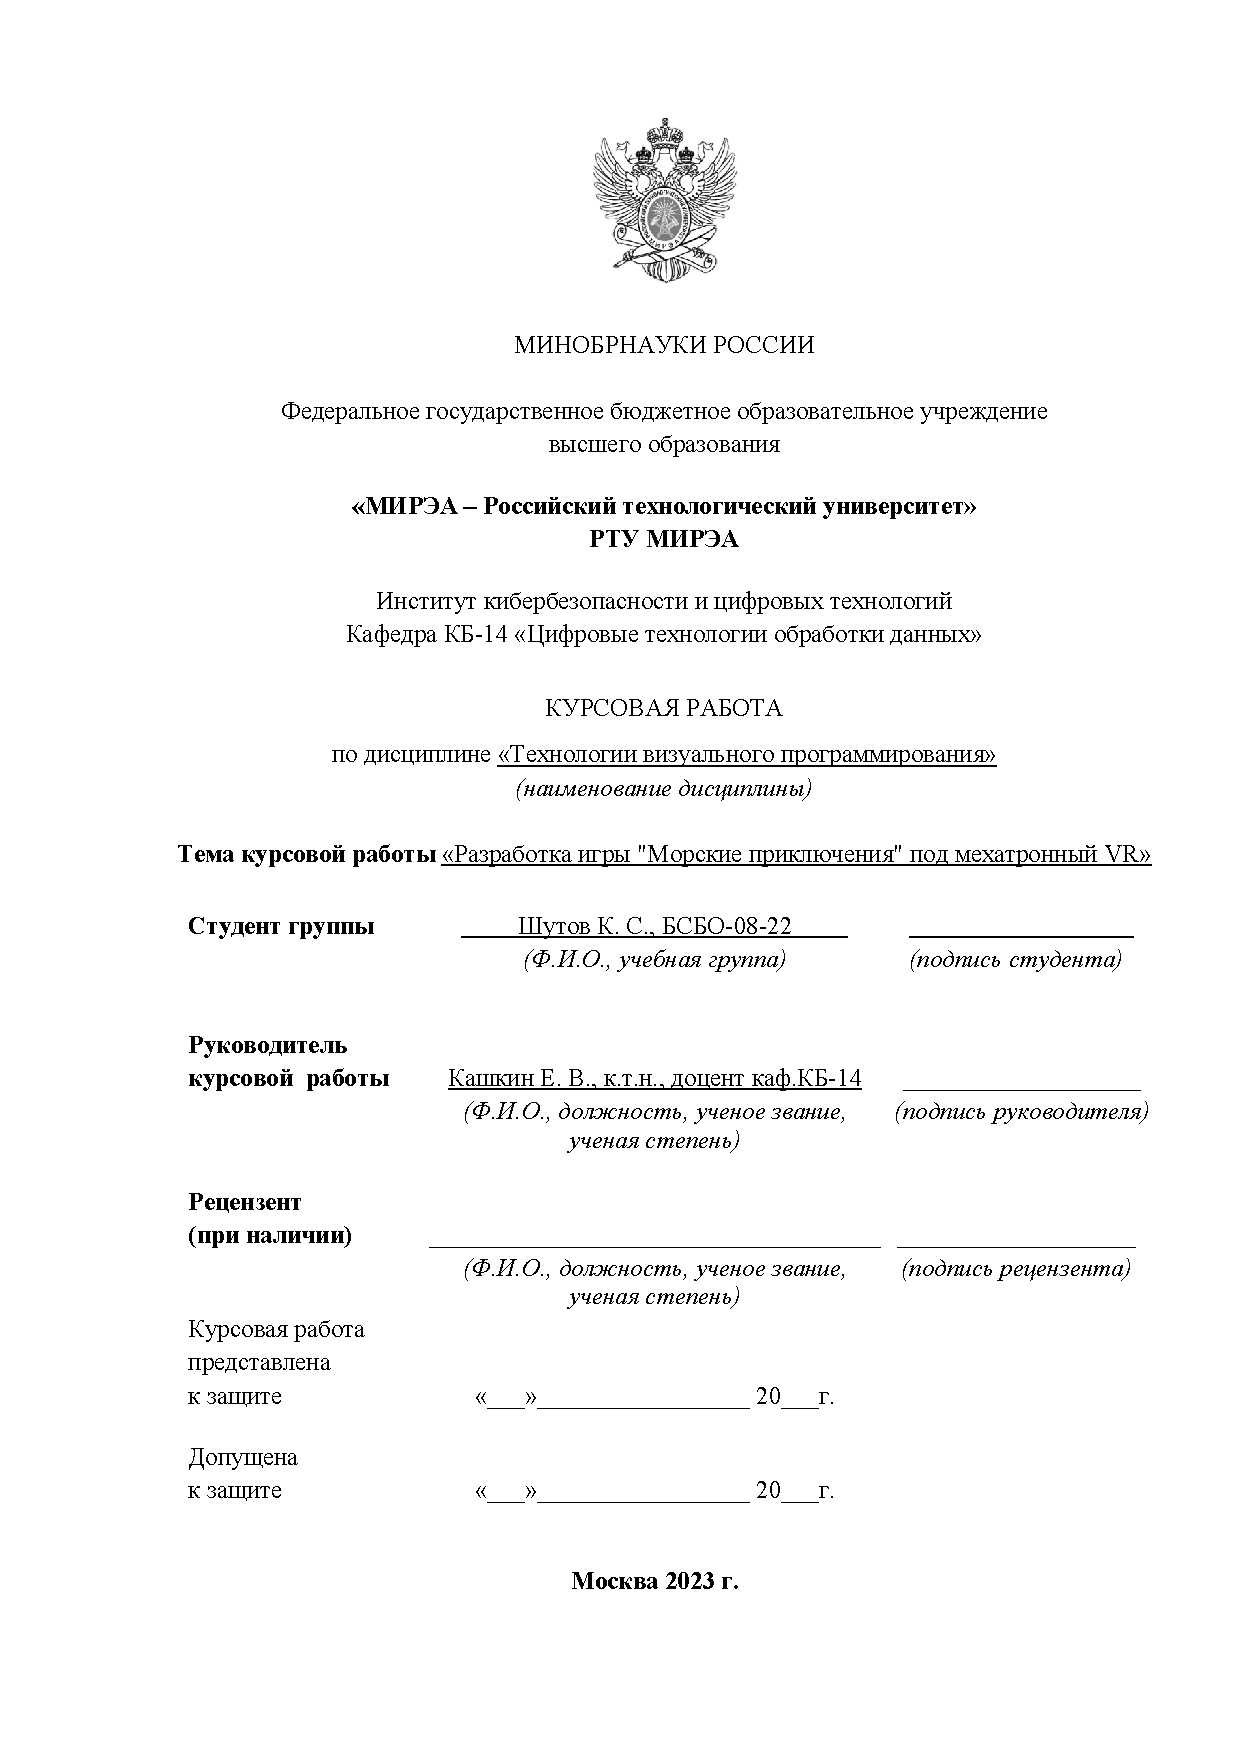
\includepdf[pages=-]{../../TitlePage.pdf}	


\includepdf[pages=-]{../../TaskPage.pdf}	

\tableofcontents

\section*{Введение}
\phantomsection
\addcontentsline{toc}{section}{Введение}

Игры являются актуальным и популярным видом время провождения в современном мире. Они стали неотъемлемой частью культуры и развлечения доступной на различных устройствах. Более того, развитие технологий позволяет создавать все более захватывающие и реалистичные игровые миры. В настоящее время помимо привычных нам устройст для запуска игр таких как компьютер, телефон, игровая консоль есть и другие, позволяющие расширить доступные игровые возможности, такие как технологии мехатронного управления и виртуальная реальность.

Целью данной курсовой работе является разработка игры "Морские приключения" с использованием технологий мехатронного управления и VR.

Игрок будет играть за персонажа, управляющего подводной лодкой, которому нужно догонять морских существ обитающих в аквариуме.

\begin{itemize}
	\item[] Во время разработки планируется провести:
	\item проектирование концепции игры;
	\item подбор ассетов для конечного продукта;
	\item моделирование игрового пространства;
	\item разработка основных игровых механик;
	\item замена грейбокс моделей на подобранные ассеты;
	\item прототипирование искусственного интеллекта морсих существ и настройка их анимации;
	\item продумывание мотивации для игрока;
	\item тестирование и отладка игры.
\end{itemize}

Особое внимание будет уделено виртуальной реальности, что позволит погрузиться в игровой мир, предоставляя уникальный опыт, который нельзя получить в традиционных играх. Одним из главных его преимуществ является то, что игра является уникальной благодаря использованию технологии мехатронного управления.

\begin{itemize}
	\item[] Будут пройдены этапы разработки игры, такие как:
	\item изучение существующих аналогов;
	\item создание концепции игры;
	\item реализации конечного продукта.
\end{itemize}

\section{Теоретическая часть}

Моя теоретическая часть.

\subsection{Мой подраздел}

Мой подраздел.



\section{Практическая часть}

Моя практическая часть.



\section*{Заключение}
\phantomsection
\addcontentsline{toc}{section}{Заключение}

Моё заключение.



\begin{thebibliography}{99\kern\bibindent}
	\bibitem{bib:mybook} Моя книга.
	\bibitem{bib:mybook2} Моя вторая книга. 
\end{thebibliography}



\appendix

\section{Моё приложение}

Моё приложение.

\section{Моё второе приложение}

Моё второе приложение.


	
\end{document}